\documentclass[14pt]{article}
\usepackage{graphicx} % Required for inserting images
\usepackage{appendix}
\usepackage{csvsimple}
\usepackage{float}
\usepackage{placeins}
\usepackage{minted}

\title{The Performance of Water Rockets}
\author{Callum Lin \& Andrei Oprea}
\date{April 2025}

\usepackage{fontspec}
\setmainfont{Arial}
\usepackage{pgfgantt}
\usepackage{hyperref}
\hypersetup{
    colorlinks,
    citecolor=blue,
    filecolor=blue,
    linkcolor=blue,
    urlcolor=blue
}
\setlength{\parindent}{0pt}
\usepackage{parskip}
\setlength{\parskip}{1em}
\begin{document}
\pagenumbering{arabic}

\maketitle
\tableofcontents
\section{Planning the project}
\subsection{Our Aims and objectives}
The aim of this project was to investigate how changing the volume of water for a water rocket would affect the performance of the rocket.

We considered our aim complete if we:
\begin{itemize}
    \item Found the trend between the volume of water in a water rocket.
    \item Found the optimum volume of water for the water rocket to achieve maximum performance.
    \item Compared our results with our hypothesis and other sources.
    \item Explained the trend between the volume of water and performance of water rocket.
\end{itemize}
Our objectives were as follows:
\begin{enumerate}
    \item To have chosen suitable metrics for measuring the performance of water rockets.
    \item To have designed and carried out a suitable experiment at varying volumes of water.
    \item To have analysed our data including trends, graphs and sources of error.
    \item To have compare our results with our hypothesis and other sources.
    \item To have broadly discussed and explained our trend.
    \item To have evaluated and reflected on our experiment, its wider implications and what we could have taken away from it.
\end{enumerate}
\subsection{Wider Implications}
The flight of model water rockets is simple yet complex. The four basic forces of thrust against drag, lift against weight are key considerations when designing a rocket - yet each component is made up of various more complex aspects all interacting with itself consisting of many interacting forces and equations including air pressure, hydrostatic pressure, laminar \& turbulent flow as well as less obvious forces such as adiabatic expansion.

Our experiment would be using these textbook theory build upon by previous authors and extending it to another domain. We believe that a model would be very useful towards helping verify these complex interactions in a new niche -- though often unexplored environment.

Furthermore, our experiment is not only limited by its scope, as a water rocket produces thrust, this experiment is applicable to many other areas such as aerospace, spacecraft and planes which all work on the same principle as water rockets.

Our results are also important where they could be used to successfully validate models such as those used in the field of aerospace, where having real world data to validate and fit models provides confidence and the necessary data required to ensure maximum performance/efficiency characteristics of real world rockets.


\subsection{Different Methods to Run the Project}
Before we started our project, we considered many varying approaches and thoroughly considered their pros and cons.

We had already narrowed down all our different approaches to completely independent work as our school was unable to allow us to shoot water rockets inside of school premises due to safety concerns.
Additionally our school was unable to provide materials so we had to finance equipment and apparatus.

For our experiment regarding water rockets, our first course of action was to obtain said rocket, we considered the following approaches:
\subsubsection{Option 1: 3D Print own rocket at school/home}
\paragraph{Positives}
\begin{itemize}
    \item Allow for the greatest amount of flexibility with the ability to change prints later if required.
    \item Allowed for more experimental freedom as we would be able to easily replace parts.
    \item Allow for a more lightweight and cheap design
    \item Allow for experiments to be carried out in parallel as two copies would allow the team members to be able to conduct the experiment at the same time.
\end{itemize}
\paragraph{Disadvantages}
\begin{itemize}
    \item We would be directly responsible for making a design that worked and provided enough stability in the air, when others have already done that.

\end{itemize}
The advantages seemed to outweigh the disadvantages so after careful consideration we had started to plan for using a 3D printer instead.\\
However we faced a fatal flaw, we lacked the resources to obtain a rubber seal and hose at reasonable cost which would be fatal for our experiment -- thus we had no choice but to abandon option 1.
\subsubsection{Option 2: Buy a kit of Amazon}
\paragraph{Positives}
\begin{itemize}
    \item Premade kit so we knew our experiment would work.
    \item The aerodynamics and stability of the water rocket would be guaranteed.
    \item Cheaper than obtaining a 3D printer.
    \item Time investment would be less compared to option 1.
\end{itemize}
\paragraph{Negatives}
\begin{itemize}
    \item Less control over fine details of the rocket.
\end{itemize}
On the whole, while this approach has fewer advantages compared to option 1, we were satisfied with the advantages provided by this approach and we believed the negatives did not hold much weight. 
\\In the end, we went for this method.
\\\\
Now that the method of obtaining the rocket was sorted out, the measurement for determining the performance of the rocket was tested out.
\subsubsection{Option 1: Measure the height of the rocket}

This method would require us to launch rockets and measure the maximum height the rocket reaches -- using this as its measure of performance.
\paragraph{Positives}

This approach would be the most direct approach to measure the performance of the rocket --  in this case optimising for height reflects many real life rocket launches and model rocket launches were height is optimised.
\paragraph{Negatives}

While this approach initially appears to be the best approach, we found several issues. 
We thought about using string/twine attached to the rocket to accurately measure the height of the rocket, but this would be confounding as we would have to keep the string taut against the force of thrust which would be impossible to quantify. 

Furthermore, using twine for a distance of ~20 metres would cause damange to the twine and result in the twine knotting itself leading to a limited number of trail runs, which are again invalid due to the presence of the taut string acting against the force of friction.

We knew we could not use twine because of this, we knew it was impossible to measure with any degree of accuracy the final height of the rocket without buying expensive equipment such as an accelerometer and associated proprietary connection ports -- this option was off the table as:
\begin{itemize}
    \item We lacked the funds needed for even the cheapest accelerometers especially after knowing we would have to buy the water rocket kit already.
    \item We were unable to find a suitable mount point to the rocket even if we did manage to acquire an accelerometer as the nozzle was at the bottom, the sides would unbalance it and cause a torque force which we believed could not even be counteracted well enough by a static counterforce as it would still be in a state of unstable equilibrium
    \item We were unable to guarantee the safety of our equipment as without a parachute, the accelerometer would suffer very high impact forces. 
    \item Attaching an accelerometer would increase the momentum and therefore increase the impact force of the rocket when it fell to levels we felt unsafe about.
    \item We lacked any resources to attach/mount the accelerometer and we lacked prior experience with electronics hardware making the likelihood of catastrophic failure higher.
    \item Would require longer and more error prone analysis of data.

\end{itemize}
Even if we overcame these difficulties, the modification would increase our chances of failure and introduce a few more (mount point, parachute, data-analysis, electronics) uncertainties threatening our experiment. 

For this method, we did not foresee any way to measure the height in a way that could possibly eliminate or reduce the chance of bought equipment (accelerometer or transmitter etc.) facing significant damage; meaning in all circumstances, we believed the disadvantages heavily outweighed the advantages. 

For these reasons above, we did not continue with option 1.
\subsubsection{Option 2: Measure the mean time taken for the rocket to fall}
This method is similar to option 1 with one main modification; timing the time the rocket is in the air the from launch to the landing.
\paragraph{Positives}
\begin{itemize}
    \item The independent variable, time, would be much easier to measure and time compared to say height or speed.
    \item Would not require any further investment of equipment other than the water rocket kit which we made already decided must be bought.
    \item Relatively straightforward compared to option 1.
\end{itemize}
\paragraph{Disadvantages}
\begin{itemize}
    \item This indirect measurement might not be what is normally correlated with the performance of said rocket.
    \item Would also require a lengthy, and perhaps more error prone, analysis of our raw results before they could be used.
\end{itemize}
We believed that option two struck a balance between the positives and negative aspects of this approach. It was very likely this method would succeed as it did not require any further manufacturer unsupported modifications of our water rocket.
\subsubsection{Option 3: Launch the rocket horizontally}
This method would require us to time the rocket as a travelled a set horizontal distance or to measure the distance the rocket travels down the field. 

We saw that there were many advantages associated with this method, but we believed that the disadvantages represented a fatal flaw to this method.
\paragraph{Positives}
\begin{itemize}
    \item This approach allows us to keep each run far more consistent, as the effects of wind and other external factors are kept at a minimum.
    \item Distance could be objectively measured using this approach compared with the others which had no way of measuring distance travelled at all.
    \item Would make our literature search far easier as many people have used distance as a better measurement of rocket performance compared to time.
    \item Distance would align better with traditional rocket performance given that in most circumstances, the height of the rocket is maximised rather than the time spent in the air.
\end{itemize}
\paragraph{Negatives}
\begin{itemize}
    \item At different volumes of water, the optimum angle to shoot it at would change and if we shot them horizontally, the frictional forces would be different.
    \item The force of friction would also increase substantially at different water volumes.
    \item The rocket, while still affected by gravity, would not be accelerating downwards at \(9.81ms^{-2}\)
\end{itemize}


Because there is no way to ensure the validity of our experiment and the forces experienced by the rocket were the least representative of all the methods for launching the rocket, we could not continue with option 3 -- leading to option 2 being the best method here.

Now that we had decided on our practical experiment we started to look for ways to compare our results with the literature. We knew that while using option 2 to measure the mean height reached by the rocket was the best method, there were serious drawbacks. Most of the established literature was focused instead of measuring the height reached by the rocket, as it was the obvious thing to measure. Because of this, we used a combination of previous work as well as using online water rocket simulators as a model to compare and contrast our results with.

\subsection{Project Plan/Method}
Our first course of action was to establish and set up our plan and timeline for our project. We carefully reviewed the pros and cons of each method, cost was a prohibitive factor so we decided that buying a kit of Amazon would the best course of action as further explained above. 

We also believed that measuring the time taken for the rocket to launch would also be the best method of determining the performance of the rocket as it is more likely to succeed and would align better with out aims, allowing a good balance between positive and negative aspects of our experiment. 

We decided to use audio recordings and video recordings as this reduced human error as much as possible, also allowing for reply of data leading to greater confidence in our results.

\subsubsection{Practical Experiment}
Our experiment was set up as follows:
\begin{itemize}
    \item A 1L Coca-Cola bottle was stripped of its label with the cap partially broken off with a weight of 39g. see \cite{2}
    \item A paper scale of negligible mass was attached to the bottle for internal verification of volumes.
    \item A water bottle rocket kit was bought of Amazon.  \cite{3}
    \item A bicycle pump was bought of Amazon.
    \item The plastic cover of the water rocket kit was screwed onto the cap of the water bottle. (as shown in Figure~\ref{fig:bottle-cap})
    \item Assuming the bottle is upright, the 3 fins were attached by sliding them into the slots up to down. (as shown in Figure~\ref{fig:bottle-fins})
    \item The provided yellow plastic tubing was attached to the value fully. (as shown in Figure~\ref{fig:tubing-pump})
\end{itemize}
The following approach was taken:
\begin{itemize}
    \item Known volumes of water was weighed out using either a measuring jug or balance.
    \item This water was poured into the bottle.
    \item The plastic seal was reattached to the bottle. (as shown in Figure~\ref{fig:full-setup})
    \item The bottle was placed on a flat surface with the fins touching the ground.
    \item A video/audio recording was taken
    \item The pump was pumped.
    \item The pressure overcame the valve and the rocket shot up (and start a stopwatch if required)
    \item Listen to the rocket land (and stop the stopwatch if required.
    \item End the video/audio recording.
\end{itemize}
Additional optional steps could be taken for example, by attaching a paper scale to the bottle of negligible mass <0.5g, or by using a scale instead of a balance. 

In the actual experiment we found these steps to be useful visual guides, however we found it did not provide any sort of tangible benefit, so it was soon removed due to natural wear and tear. \\This did not affect our results in any way as the negligible mass accounted to an equivalent of less than 0.5 mL of water, which was far under the apparent human error in our experiment. We
\begin{figure}[h]
    \centering
    \includegraphics[width=0.38\textwidth]{Bottle with cap.jpg}
    \caption{Bottle with cap}
    \label{fig:bottle-cap}
\end{figure}
\FloatBarrier

\begin{figure}[h]
    \centering
    \includegraphics[width=0.38\textwidth]{Bottle with fins.jpg}
    \caption{Bottle with fins}  
    \label{fig:bottle-fins}
\end{figure}
\FloatBarrier

\begin{figure}[h]
    \centering
    \includegraphics[width=0.5\textwidth]{Tubing and pump.jpg}
    \caption{Tubing and pump}
    \label{fig:tubing-pump}
\end{figure}
\FloatBarrier

\begin{figure}[h]
    \centering
    \includegraphics[width=0.5\textwidth]{Full setup.jpg}
    \caption{Full setup}
    \label{fig:full-setup}
\end{figure}
\FloatBarrier

\subsubsection{After the Experiment}
Analysis of raw data:
\begin{itemize}
    \item Videos and audio was analysed by sound/movement to determine the time the rocket was in the air.
    \item Graphs and conclusions were drawn out
\end{itemize}
Comparison of data:
\begin{itemize}
    \item The water rocket attributes were taken except pressure which could not be experimentally tested.
    \item A suitable site was found in which we could take data of volume of water against mean time until touchdown.
    \item Data was scraped from the site for further analysis
\end{itemize}
After the data collection, we aimed to be able to:
\begin{itemize}
    \item Explain our results.
    \item Draw conclusions.
    \item Writeup our report.
\end{itemize}
Our rationale for using a online simulator would be to effectively increase our trust in our results as we saw that there was a lack of prior work in the area, that way, we could see how the best line curve correlates with the equations governing the laws of motion.

Furthermore, using this method would provide an adequate level of difficulty allowing us to test out skills benefiting our knowledge of the sciences. We also believe that using a model would help increase the impact of our work.

\subsection{Plan and Timeline}
Our work was split into six distinct stages: experimental research, practical work, data analysis, secondary source analysis, overall results analysis and writeup.

Most of these stages occurred concurrently at the same time such as analysis of data right after each trial. 

The reason for this was practically as water rocket launches were limited to day time hours, which meant we often had time left over to check for second sources and analyse our partial data.
\subsubsection{Experimental Research}
This initial section was conducted at the start of our CREST Project over the course of several months.

Early September: Initial ideas for this project were floated and we looked into the practicalities of this experiment and multiple others such as pendulum motion, electrolysis and insulation material.

September 24th: Our plans and research was submitted to our schools CREST organiser and we brainstormed ideas and apparatus for our experiment.

October 5th: Our school's CREST organisers approved our plan, thinking it held the potential to make an interesting CREST research project. We had already previously conducted research on the apparatus needed for our experiment.
\\
Mid October: An individual in our group bought the rocket kit off Amazon and  at this point in time we were still unsure of what method we would use to measure the performance of the rocket, so we continued searching for inexpensive equipment such as accelerometers and Bluetooth GPS receivers. 

Start of November: The pump was bought by another individual in our group which arrived many weeks later.

End of November: A limited trial run was conducted to see the performance, from this it was evident that it was impossible to measure the height the rocket reached with any degree of accuracy without equipment such as the aforementioned accelerometer or Bluetooth GPS, now, we started to consider measuring the mean flight time instead.\\

December to February: During this time,  we conducted further secondary source research. We also continued searching for accelerometers and Bluetooth GPS's until this was abandoned due to many issues we foreseen would arise -- these factors were listed in more detail in "1.3 Different Methods to Run the Project" above.\\

During this time, the cold weather made is physically impossible for us to conduct any practical work which was an unforeseen obstacle leading to us having to reevaluate our plan of action to keep up with the ever pressing deadline.
\subsubsection{Practical Work}
For our practical work, the cold winter meant we had a significantly shorter amount of time to conduct the experiment than we would have liked. This was obviously unfortunate but we had discussed this together during the winter months when the cold temperatures prevented any runs from occurring.

January to February: We tried to conduct multiple experiments during this phase but the extreme temperatures outside prevented my fingers from being able to manipulate the apparatus and the lack of daylight made conditions less than ideal for our experiment. We were not able to conduct any practical experiment, though we did give a best effort, during this time. 

Start of March: During this period, as school had started and it was still relatively dark, midges and the lack of daylight hours were a persistent problem as we were unable to do it during school hours. This limited our possible experimental days to only Saturday and Sunday.
This was very conflicting with our schedules as one of the group members had Chinese School where they were doing their qualifications and another had out-of-school extracurricular activities which they had attended for several years on Sundays. As the group members could only exchange apparatus during school hours some time was unfortunately not utilized at all.

Taking this into account, we each dedicated several hours each day towards practical work, with even more dedicated towards the project as a whole, which was the most we could physically do given the fact that the daylight hours were still limited and we had to attend other non-negotiable commitments at that time. It was during this stage that the stages started to do these sections concurrently as we were aware the daylight and environmental factors were against us. 

March 8th: An experiment was conducted for a total of 1.5 hours with a time split of 1 hour doing the experiment was audio files available from this time period and 15 minutes travel and setup requirements both ways. As all our experiments required common setup and took approximately the same amount of time (due to physical constrains and safety concerns associated with carrying out repetitive movements for several hours in a row which limited the maximum amount of time we could conduct the experiment for), to be more concise, this fact and the previous ones mentioned in this paragraph will be only briefly mentioned in the future.\\See Appendix A [\ref{Appendix A}] for the set of results for this date.

March 9th: Another run was conducted for a couple more hours. Again setup took a similar time and our results are also available in Appendix A [\ref{Appendix A}].





\subsubsection{Data Analysis}
This was the most straightforward part of our project, after each practical experiment was concluded, we replayed the audio/video multiple times and measured the time from launch to touchdown and wrote down this value. Mean values were also calculated.



\subsubsection{Secondary Source Analysis}
This section was conduction in parallel with our practical experiment, as we often did not have the daylight hours to conduct the practical experiment and the practical experiment was running late due to the effect of the winter temperatures delaying our project.

February and March: Originally our plan was to create our own model, we spent a lot of time on this (~4 hours each day) several days a week, but to no avail. Even when we got a working prototype working, the number of bugs in it gave us reason to doubt the efficacy of our simulation given the fact that online simulations were better tested and used than ours.

Match 10th: This day, we took information regarding the bottle, and we tried but failed to establish the pressure required for the rocket to launch, due to a lack of equipment and the rubber valve expanding on contact on water increasing the effect of friction so the pressure was higher when measured, sometimes explosively higher. \\
Measurements we took were bottle nozzle diameter, bottle diameter, mass of the rocket and the total volume of the rocket. This can be found in Appendix B [\ref{Appendix B}]

April: After the failed try, we found an online source which was very popular and we found, after testing multiple ones, to be the one with the fastest and most transparent results as compared to other source obfuscated websites.\\
We used the website by (Deen Wheeler and George Katz [website] 2017-2020) \cite{6} and created code to scrape it as it only showed water volume vs height and not water volume vs mean flight time.

\subsubsection{Overall Results Analysis}

March - Present: Now that we had both our results and our secondary source, we compared the two trends below.

\subsubsection{Writeup}
March - Present: This section required us to refine our writing skills and present our data. One regret we had is that some of our original data files were lost as we were unaware we should have saved them for archival purposes. Here we encountered the most difficulties often spending over 6 hours each day per person each week to complete the writeup.


\section{Throughout the project}
\subsection{Materials, Resources and people}
The project required access to a water rocket and a pump. We were able to identify a water rocket through the help of our teacher, who found
a suitable rocket which could be purchased online. Similarly, for the pump we identified and ordered a bicycle pump from online.

Additionally, we needed equipment to allow us to measure the volume of water at the experiment site. We found our own measuring jug, as well
as a 5L folding water container to hold the water. For recording the rocket’s flight times, we used  our devices.
\subsection{Underlying physics}
\subsubsection{Propulsion and Motion}
The rocket is held in place by a pump that is designed to release at a certain pressure. As air is pumped into the rocket from the pump, the internal pressure increases, eventually reaching the required pressure and resulting the launch of the rocket. Immediately, the water will be expelled downwards due to the high pressure, thus providing an equal and upwards reaction force known as thrust which will propel the rocket until all of the water is expelled. As the compressed air from the rocket is released, the volume it occupies increases, so according to the formula \(PV = constant\), the pressure inside the rocket decreases. This results in a decrease in the force which expels the water, so the rate at which water is being expelled will decrease over time. The rocket will then continue to rise until it reaches a velocity of 0 at the peak of its trajectory and it will then fall back down. The rocket's flight time can be measured, because this quantity will be related to the initial acceleration of the rocket, and this quantity serves as a measure of performance. 

The aim of finding the optimal water to air ratio is based on the principle that too much water will make the rocket heavier, while too little water means reduced reaction mass to generate thrust. The optimal ratio will produce the greatest acceleration and therefore the greatest recorded time. 
\subsubsection{Aerodynamics}
There are small disturbances in the air which may push a flying bottle of its straight path, which is why according (Nakka R., 2019), fins are required to stabilise the rocket and prevent it from veering off course \cite{4}. According to (Hall N., 2023) the fins work by producing a restoring force \cite{5}, which will counteract changes in pitch or rotation. This happens because when the rocket tilts off the flight path, the fins will pass through the air at an angle. As the fin hits the air, the air will apply
an equal and opposite force on the fin, according to Newton's third law. Since the fin is at the rear of the rocket, away from the center of mass,
the force will not only push the rocket but generate a torque that causes rotation about the center of mass (similarly to a seesaw), which will restore the rocket to its initial position.  Therefore,
to steer a rocket, the restoring force of the fins must be overcome.
The main reason for the fins being placed at the end of the bottle is to maximise torque, which results in a greater stabilising force, which is in accordance with the formula
for torque : \(T = F \cdot r\).

\section{Finalising the project}
\subsection{Conclusions}

The aim of this project was to investigate how changing the volume of water in a water rocket affects its performance. The results showed that that there is an optimal water volume that maximises flight. 

Our hypothesis was that as the volume of water increased the performance would initially increase due to greater thrust, until the optimal volume was reached. Beyond this optimal volume, the performance would decrease significantly because as the water mass became too large, the thrust generated would no longer be sufficient to overcome the rocket’s weight.

Our data shows a similar trend until the optimum volume, because the flight time increases as the volume of water increases, until it reaches a global maximum of 2.78s at a volume of water = 150 ml. After this, the flight times are all less than 2.78s, with a general decreasing trend as the volume of water increases. There are unexpected increases in flight times at volumes 200ml and 250ml and this cannot be explained by the underlying physics of a water rocket's motion, so it can be attributed to factors including insufficient repetitions at those volumes or unintended changes in the experimental setup during those runs. Specifically, an increase in performance could suggest that the valve was plugged further into the seal than the other runs, thus reducing pressure leaks, so the initial pressure at launch would be greater. Another possible explanation could be a systematic error, such as an incorrect measurement of the 200 ml and 250 ml volumes, due to low precision in measuring instruments.
\begin{figure}[h]
    \centering
    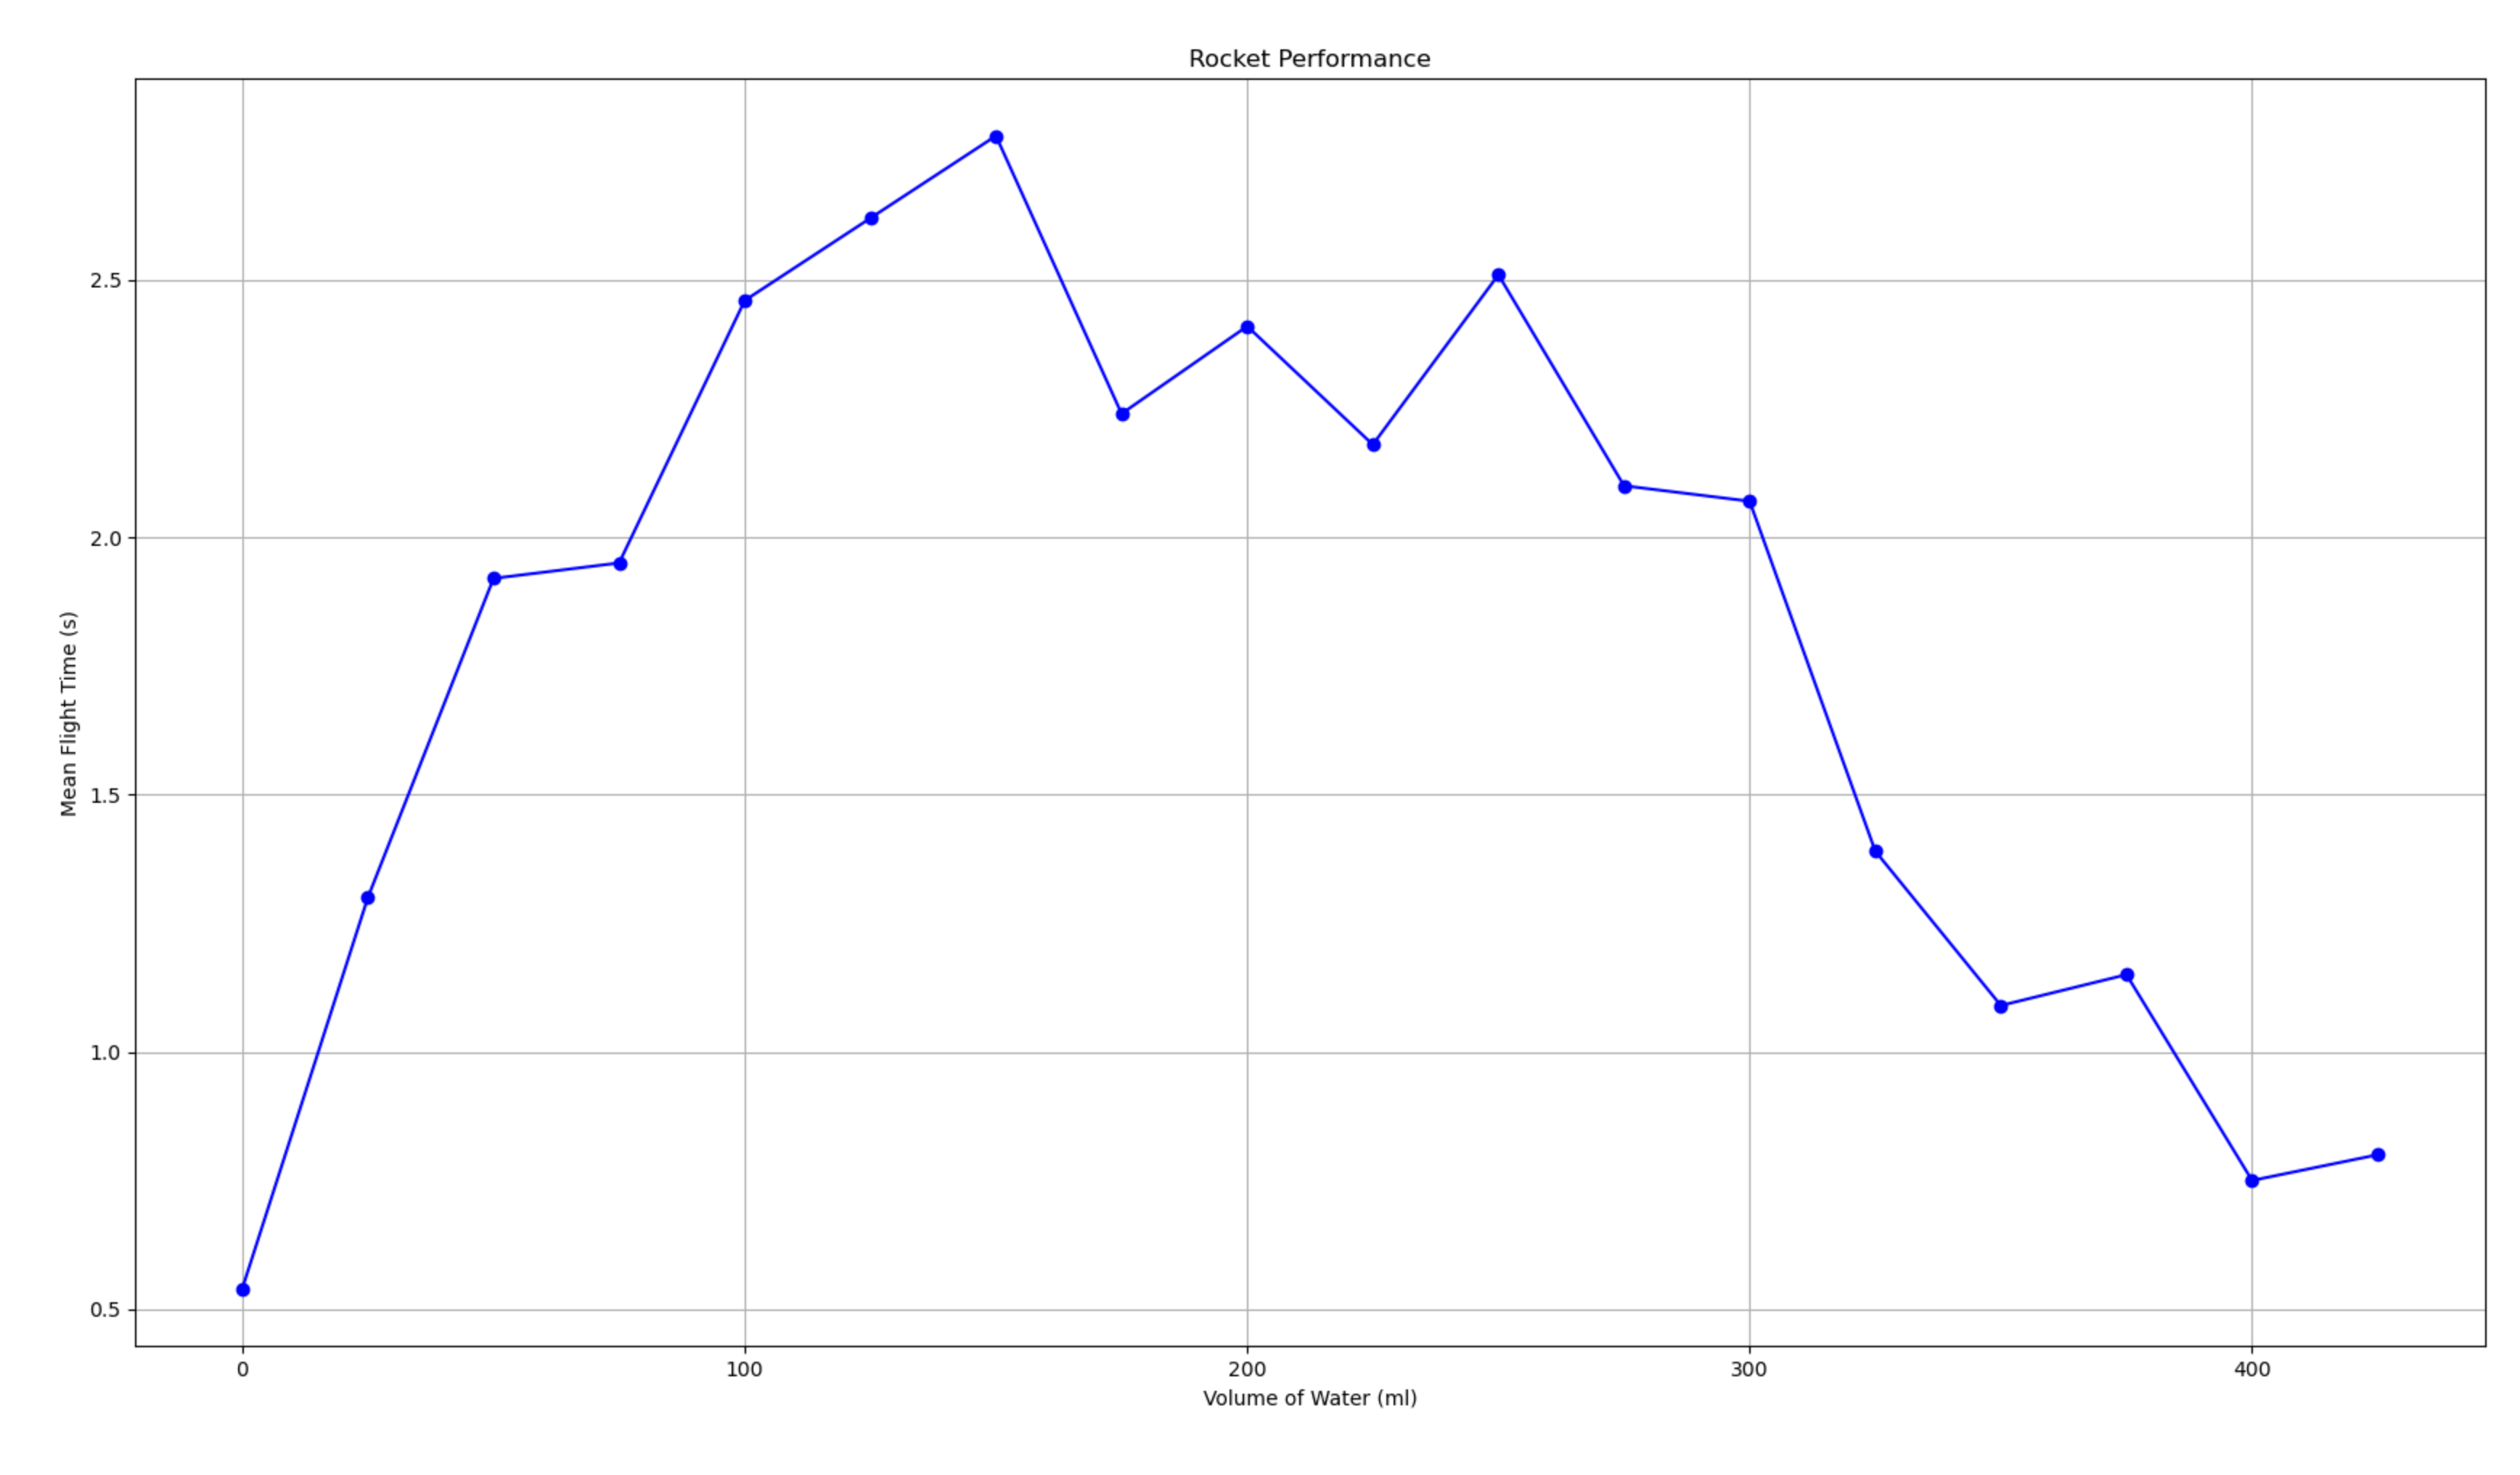
\includegraphics[width=\textwidth]{graph.png}
    \caption{Graph of results}
\end{figure}
\FloatBarrier

This aligns with our secondary source, which also had an increasing flight time towards a maximum, after which the flight times decreased. This produces a parabolic graph, which is a similar trend shown by our graph, although there are deviations at volumes of 200ml and 250ml.
\begin{figure}[h]
    \centering
    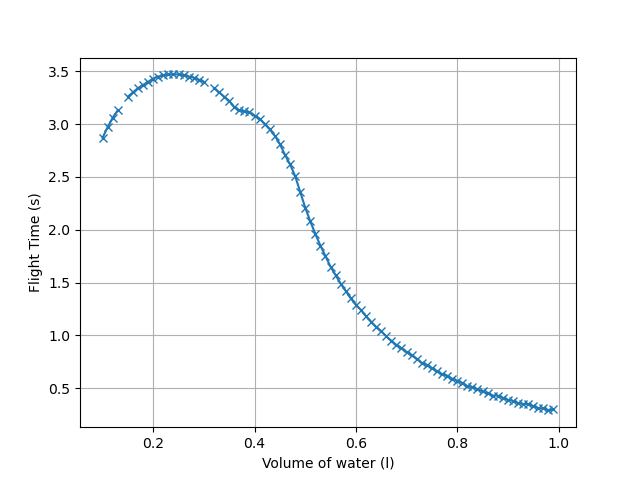
\includegraphics[width=\textwidth]{second-source.png}
    \caption{Secondary Source Zoomed Out}
\end{figure}
\FloatBarrier
\begin{figure}[h]
    \centering
    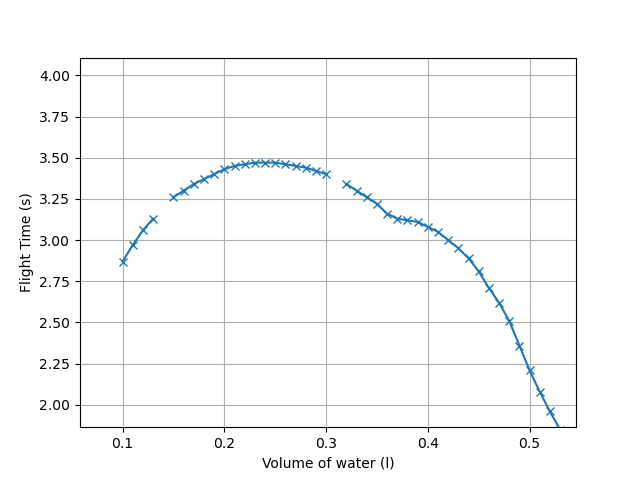
\includegraphics[width=\textwidth]{second-source-zoomed-in.png}
    \caption{Secondary Source Zoomed into our experimental range}
\end{figure}
\FloatBarrier
For our secondary source, there were a couple limitations that we wanted to make you aware of. The pressure on the website was prevented from being too low which explains why we cannot get our secondary source's time to line up with ours. \\Another issue is that their simulation due to floating point precision errors would sometime not give a result for some data points leading to missing data points. \\
Another issue would be the fact that the volume of water cannot be prevented from going lower than 0.1L, although this was a common theme among all the online simulators.\\
We still stand by our choice because we are aware that these limitations do not impact the accuracy of the result, as floating point number limitations only become an issue close to values of 0, which the simulator has rightly blocked.

For the code used to generate this see Appendix C, the graph in tabulated form is also present in Appendix C.

Using our results, and our results being bolstered by the simulation, we can confidently conclude that the best volumes to use for a water rocket follows a parabola with one side being of greater steepness, however, we find that as our range was not as extreme, for our purposes, we considered it to be an even parabola as highlighted by our secondary source zoomed into the range we did our experiment in.

For our results we found a maximum peak at 150mL at 2.78 seconds, this is in contrast to our secondary source which has their peak higher at around 0.24mL at 3.5 seconds. We believe this is because as you increase the pressure, which theirs was evident by the fact the graph was higher, the optimal pressure increases as more water will be able to be pushed out until the turning point is reached, where the extra weight is too large for the smaller increase in thrust. This was also validated by toying around with the simulator, where we saw how increasing pressure would lead to a higher peak towards the right of the graph.
 
\subsection{How our actions impacted the project}
Our decision to use method 2 in our experiment meant that the data we had to analyse was related to the rocket's total flight time, which affected how we made our analysis and explored the underlying physics. As well, it meant that we had to spent time analysing video/audio recordings with a stopwatch to record the results.

We effectively used our time such that while one member was collecting results for the experiment over a fixed period of time, the other person was researching or completing analysis of results. Through this process, we were able to efficiently produce results while working on our report.
\subsection{What we learned and further improvements to our experiment}
From our project, we learned that:
\begin{itemize}
\item To achieve maximum performance for a 1L water-rocket, 150ml of water must be used.
\item Fins are essential to ensure that a rocket remains on a straight path.
\item A simple but effective way to carry out a water-rocket experiment is to measure the rocket's flight time.
\end{itemize}
We also learned various skills including how to evaluate experimental methods by thinking about their practicality and implication on how the results are measured.
Throughout the project we also learned the importance of communication, as this was necessary to effectively share our thoughts and concerns about the experimental procedure, results and underlying physics.

Our project could have been improved by being able to perform the trials in less windy conditions, as this would reduce the effect of updraft on the rocket's flight time. To minimise the impact of external factors like wind, we spread out the launches, ensuring that no single day's weather conditions would disproportionately affect the overall results, however we believe that this did not fully resolve the issue as the change in the speed of the wind between days would have altered the results. In addition, it could have been improved by having access to more precise equipment, as the measuring jug used to measure the known volumes of water had a low degree of precision, which could cause the results to be less reliable, as a small change in the volume of water resulted in a large change in the recorded time. We think this could have been a factor affecting the results, because even with sufficient repetitions at each volume, there were unexpected results in nearby volumes. Alternatively, a measuring cylinder could be used instead of a measuring jug, as it may have closer divisions and thus less uncertainty.

Having access to a pressure gauge would improve the experiment, as it would allow us to verify (approximately) the pressure that the rocket launches at, and this is important as different release pressures would influence the recorded times. It would also allow us to enter the true value of pressure as a parameter into the simulation, thus improving its accuracy compared to the real setup. It would also allow us to determine if the rate of air pumping affected the results, since a possible but unlikely scenario could be that the rate at which air was pumped into the rocket was too fast in certain runs, resulting in a temporary increase in pressure above the release pressure and causing a release at a higher pressure than intended, therefore interfering with the results.

Finally another improvement would be to to try and find locations with more flat surfaces or more open space, as in certain areas used to test the rocket, the angle of incline provided by the surface produced unwanted horizontal motion by the rocket, which would not affect the recorded times but meant that it would be at greater risk of becoming stuck and possibly lost in nearby buildings or bushes.
\section{Project-wide criteria}
\subsection{Direction, Ethics and Safety}
\subsubsection{Direction}
Our project was mainly self directed, so we took full responsibility to prevent accidents/events.
Some parts of our project was completely unsupervised such as the scraping of our secondary source was out of our school's crest organisers expertise. 

We consulted with our Physics teacher on whether this was a viable experiment as well as reflecting with her on the various expected problems we would encounter, past this point we self directed the rest of the project checking in occasionally for advice on underlying physics and the writeup itself.
\subsubsection{Ethics and safety}
Because we used audio and video recordings to record our rocket launches, our experiment required the collection of personal information such as images, voice and possibly location. This had to be stored securely to avoid inadvertent disclosure to third parties.

To satisfy this requirement the we used strict access controls, information was only ever stored locally or on an encrypted cloud platform, in this case we used Google Drive. We avoided storing information on our school's personal accounts due to this meaning they would have full access to personal information. Using this method, we believe we had completely satisfied our privacy and ethics obligations both as researchers and legally as well.

Because it was highly recommended for us to upload video and audio recordings by our mentor, we created personal data usage forms, to allow us to send this raw data to you.\\
Because we were unaware before starting this writeup that it would be recommended for us to upload raw files, some participants did not agree to these terms so some recordings have been redacted.

Because our raw data files were incredibly large > 150MiB, and they did not fit the file requirements being an unsupported .aac format, we uploaded the files on Github instead. We informed the participants of the experiment and asked for written consent for this audio/video to be made public as CREST required these documents to be accessible. \\
One participant out of two consented meaning we were able to both respect the privacy considerations of each individual and upload some raw data as well.

A further consideration for us was the fact that images of other people/restricted information such as license plates could possibly appear.\\While this would not be illegal, as individuals have no expectation of privacy in a public place, our ethics obligated us to stop filming when a person was approaching

For our risk assessment we identified the following risks and their severity, we also identified methods to reduce this risk to an acceptable level.
Risks include:
\begin{itemize}
    \item The rocket hitting objects on impact such as cars, buildings, utiity poles etc. \\We classed this as high impact owning to the fact that property destruction is very costly and would lead to financial liability for us.
    \item Another risk was the potential for the rocket to get lost leading to both environmental damage as the bottle could pollute the environment. \\Another consideration would be that if we lost the rocket, it would not only cause significant delay to the project, but it would also be a waste of resources.
    \item A risk which we considered was the plastic water bottle blowing up, we considered this as a extreme impact, low likelihood event. \\ To mitigate these risks, in our trial run we carried out, we went to a secluded wooded place with no animals or objects nearby and subjected the rocket to extreme operating pressures by stepping on it. \\ As the rocket showed no sign of degradation at all after this event, we felt comfortable subjecting it to the manufacturer rated pressures after this. \\ A further assurance for us was the Amazon reviews with no reviews mentioning the blow up of the rocket.

\end{itemize}

\subsection{Problems we faced and how we overcame them}
During initial testing of the rocket, we found that the performance of the rocket was too great, which meant that the height it reached was high enough to get lost in nearby buildings and certain horizontal motion may have resulted in the rocket landing outside the designated experiment zone. 
\\To resolve this, we decided to reduce the performance by not plugging the hose's seal into the seal all the way in but instead half way through. This reduces performance because the valve isn't as tightly sealed, so there is reduced pressure and therefore reduced thrust. This is effective because lowering the pressure for all runs should still maintain the trend in recorded times, when compared to a higher pressure.

\begin{thebibliography}{0}

\bibitem{2}
Coke-1-litre | taste thirst [internet]. London (U.K.): Taste Thirst c2023. [Updated 2023; cited 2025 Mar 22]; [Image of Coke-1 litre bottle]: Available from: https://tastethirst.com/product/coke-1litre/
\bibitem{3}
Funtime Gifts 10657 Bottle Rocket Kit : Amazon.co.uk: Toys \& Games. Seattle (U.S.) c2025. [Updated 2025; cited; 2025 Mar 22]; [Product Listing]: Available from https://amzn.eu/d/4BXIgWf
\bibitem{6}
Water Rocket Simulator [Internet]. Air Command Rockets. 2017-2020 Available from http://www.aircommandrockets.com/sim/simulator.htm
\bibitem{4}
Nakka R. Richard Nakka’s Experimental Rocketry Site [Internet]. Nakka-rocketry.net. 2019. Available from: https://www.nakka-rocketry.net/fins.html
\bibitem{5}
Hall N. Rocket Stability | Glenn Research Center | NASA [Internet]. Glenn Research Center | NASA. 2023. Available from: https://www1.grc.nasa.gov/beginners-guide-to-aeronautics/rocket-stability/
\end{thebibliography}

\section{Appendices}
\subsection{Appendix A}
\label {Appendix A}
\textbf{Results}
\FloatBarrier
All results
\begin{figure}[h]
    \centering
    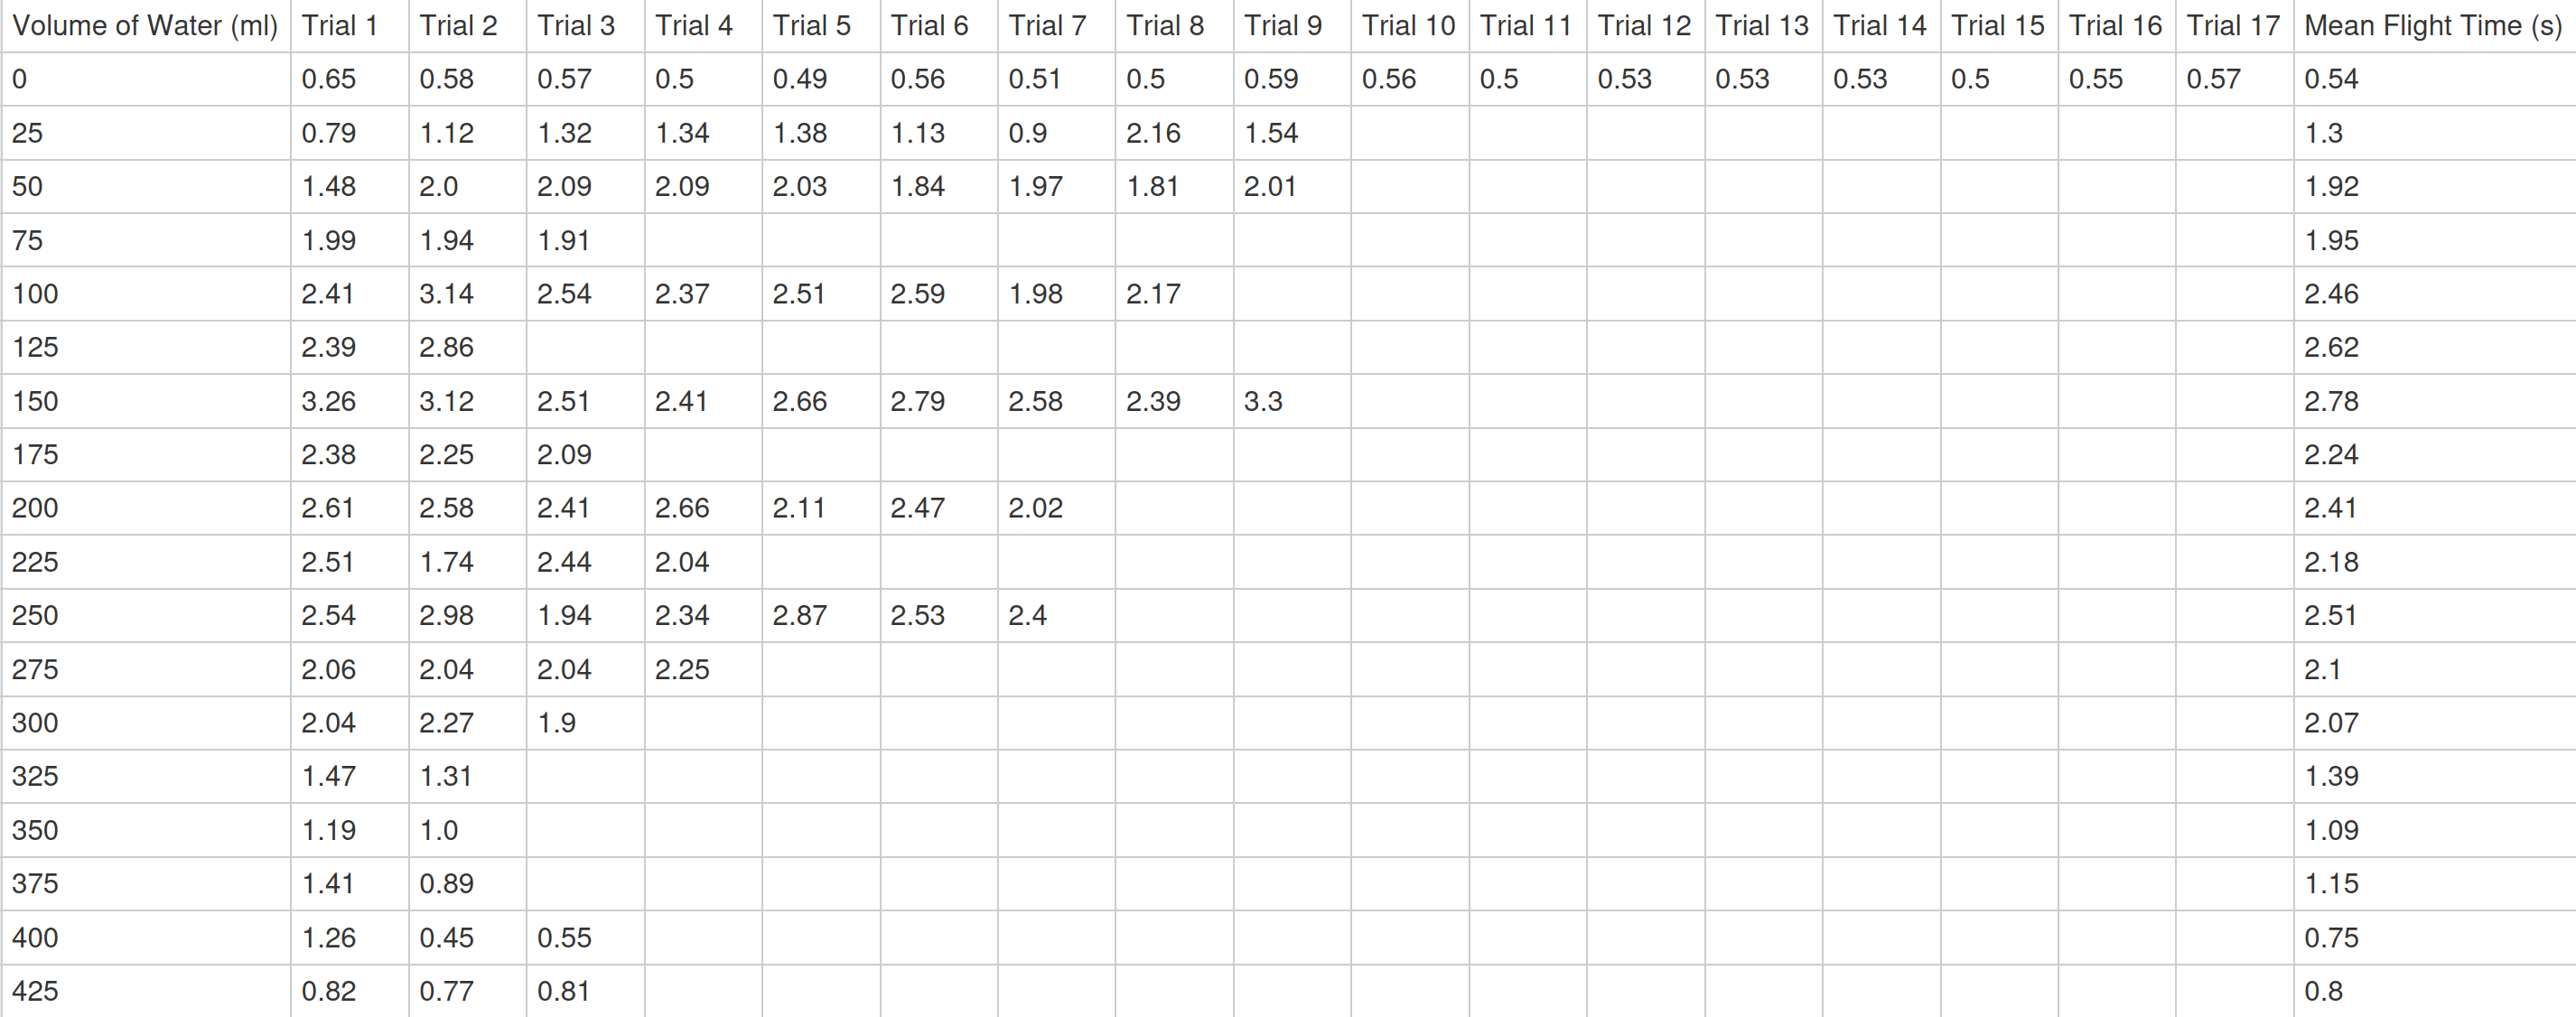
\includegraphics[width=\textwidth]{data/all_data.png}
\end{figure}
\FloatBarrier

March 8th
\begin{figure}[h]
    \centering
    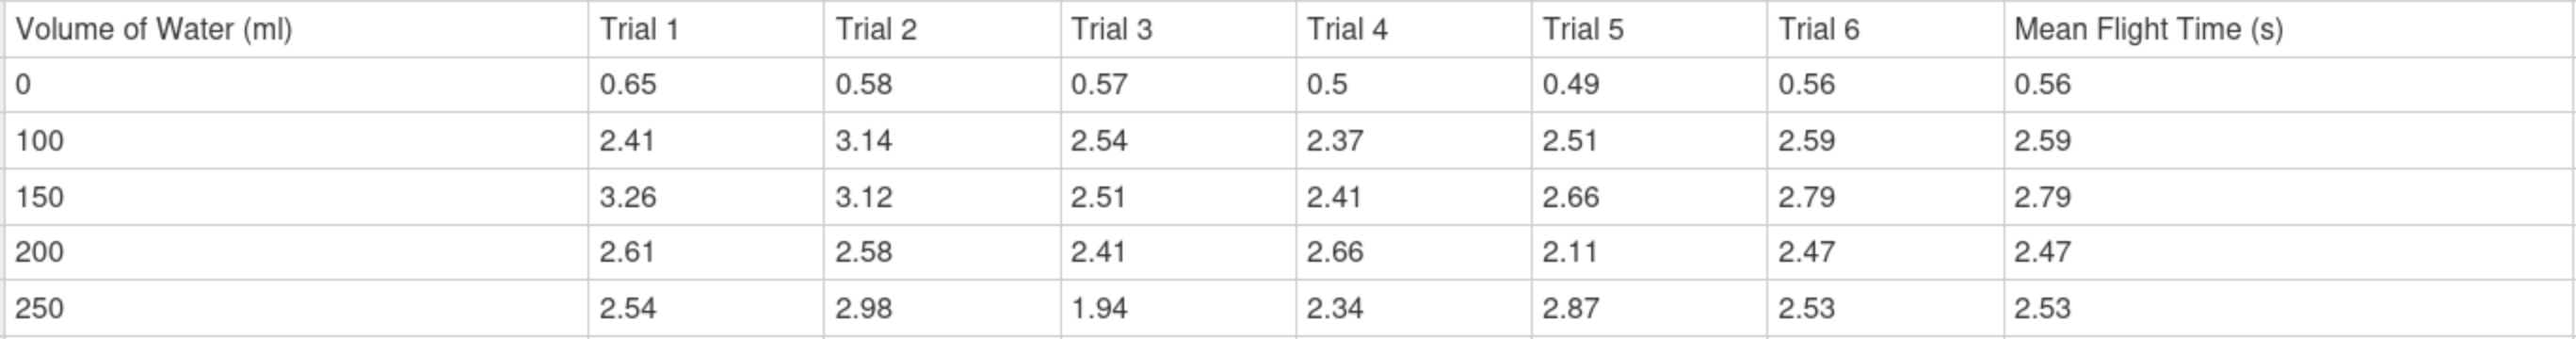
\includegraphics[width=\textwidth]{data/8th.png}
\end{figure}
\FloatBarrier

March 9th

\begin{figure}[h]
    \centering
    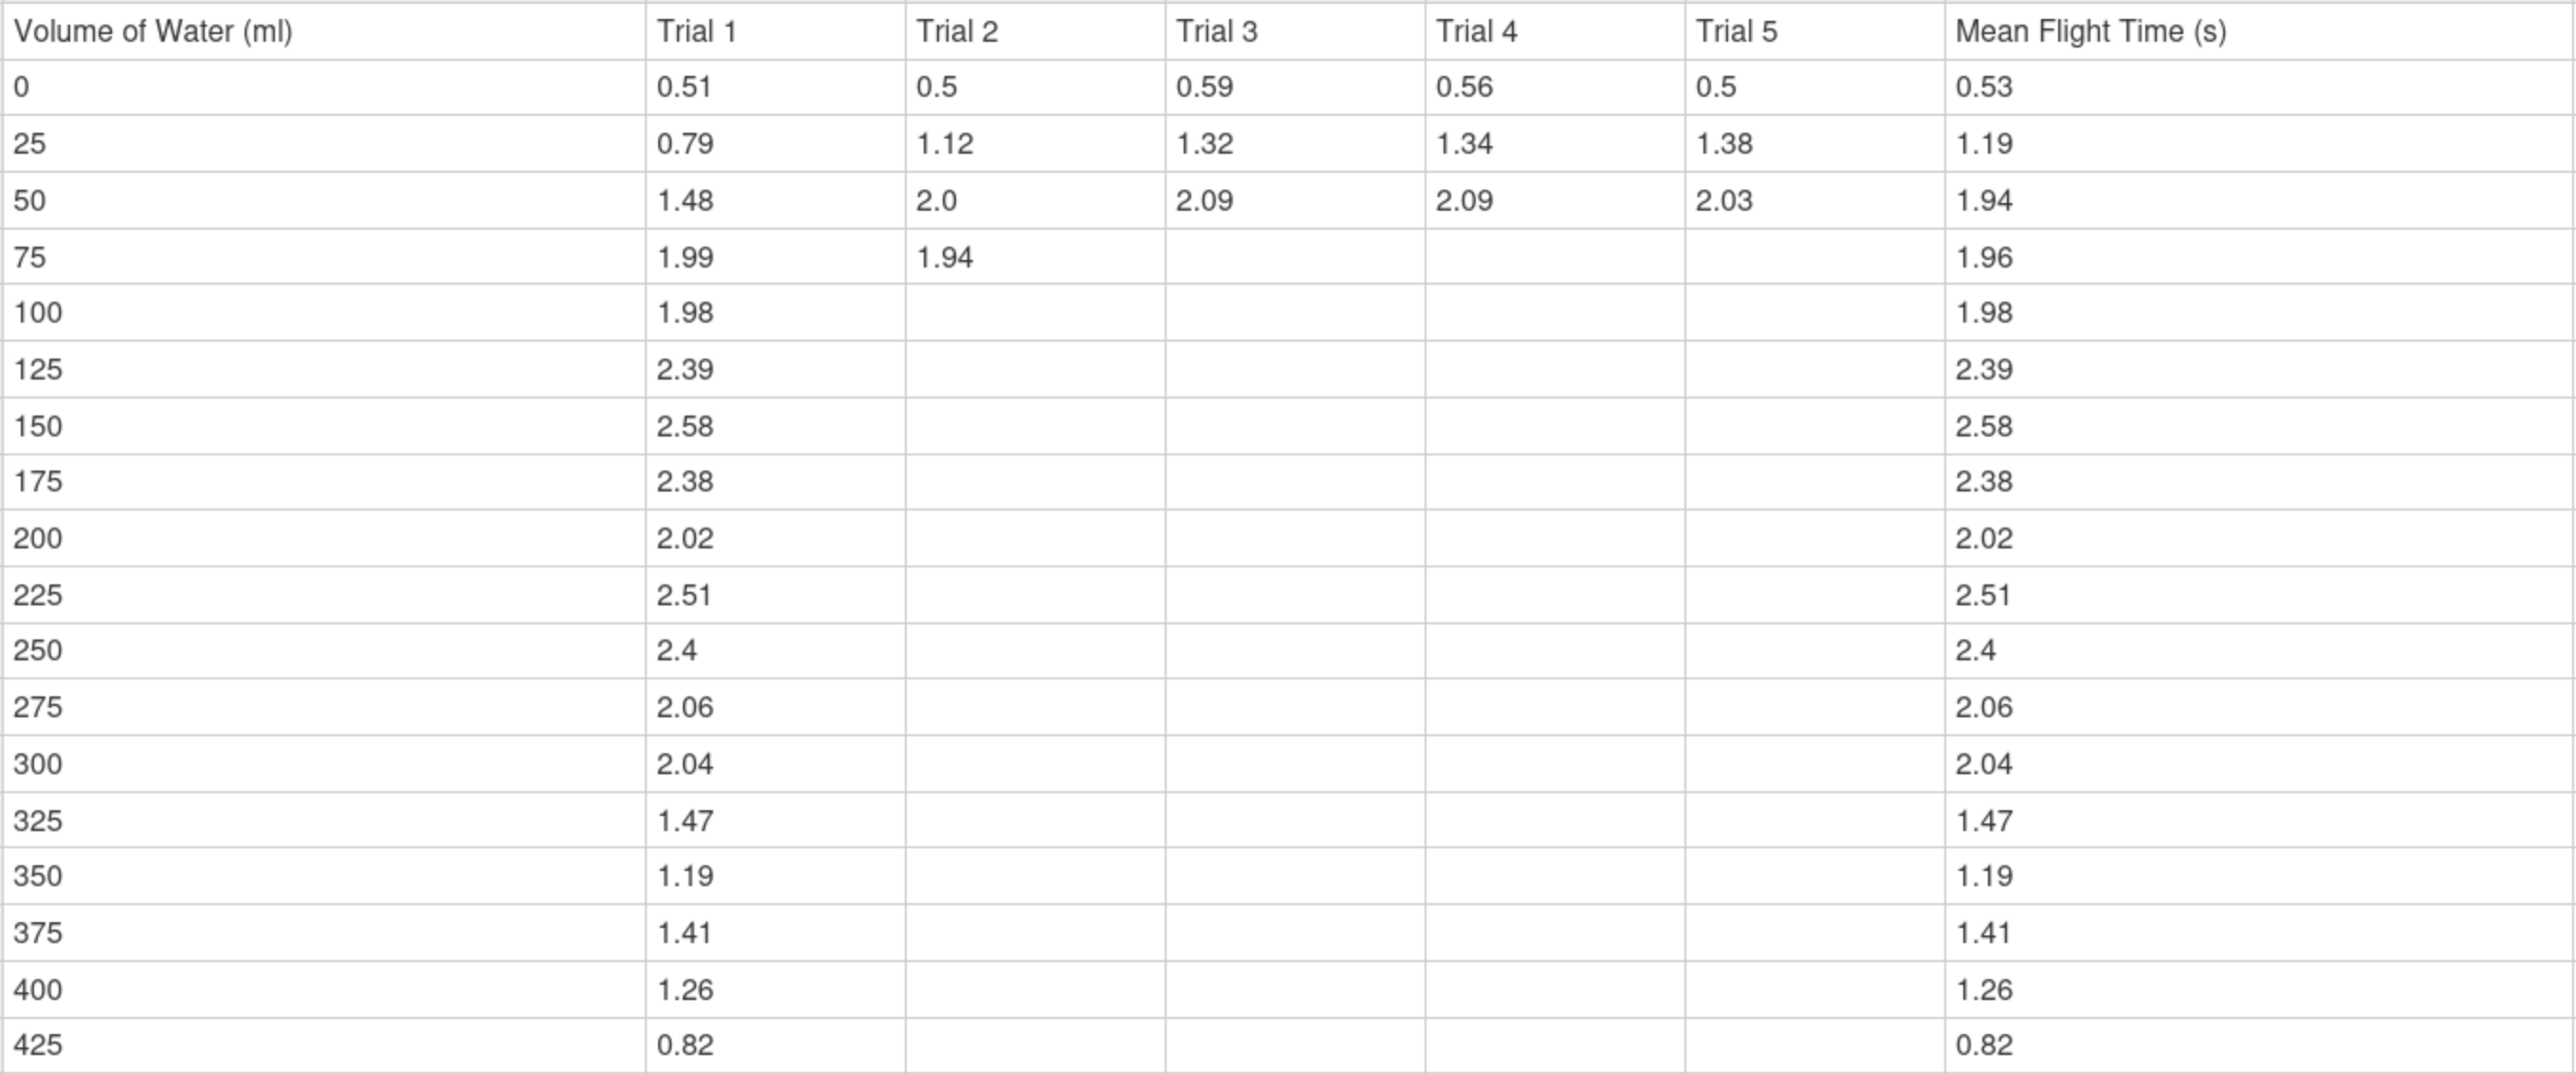
\includegraphics[width=\textwidth]{data/9th.png}
\end{figure}
\FloatBarrier
March 15th

\begin{figure}[h]
    \centering
    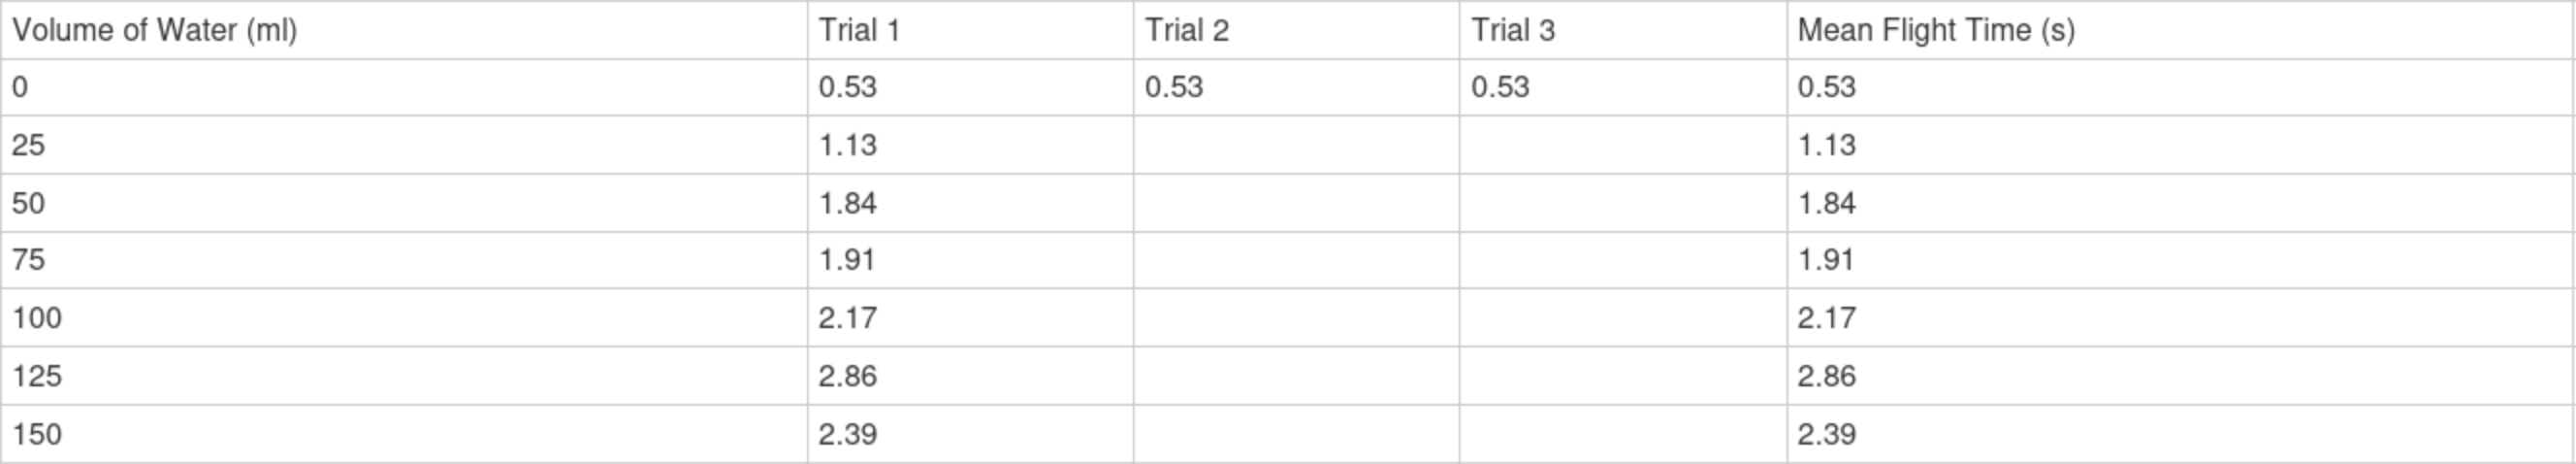
\includegraphics[width=\textwidth]{data/15th.png}
\end{figure}
\FloatBarrier
March 16th

\begin{figure}[h]
    \centering
    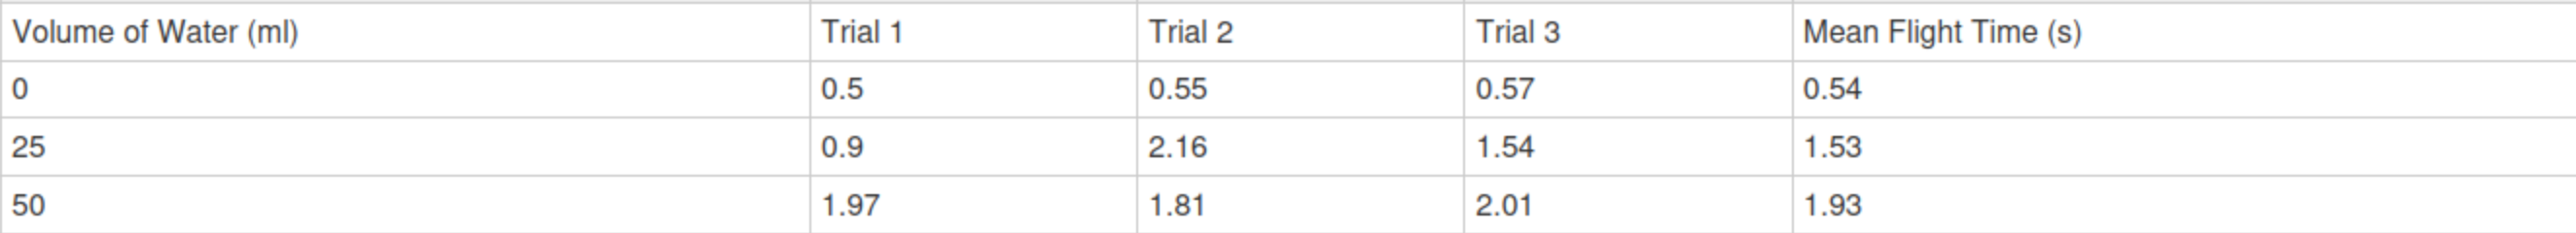
\includegraphics[width=\textwidth]{data/16th.png}
\end{figure}
\FloatBarrier

March 21st-30th

\begin{figure}[h]
    \centering
    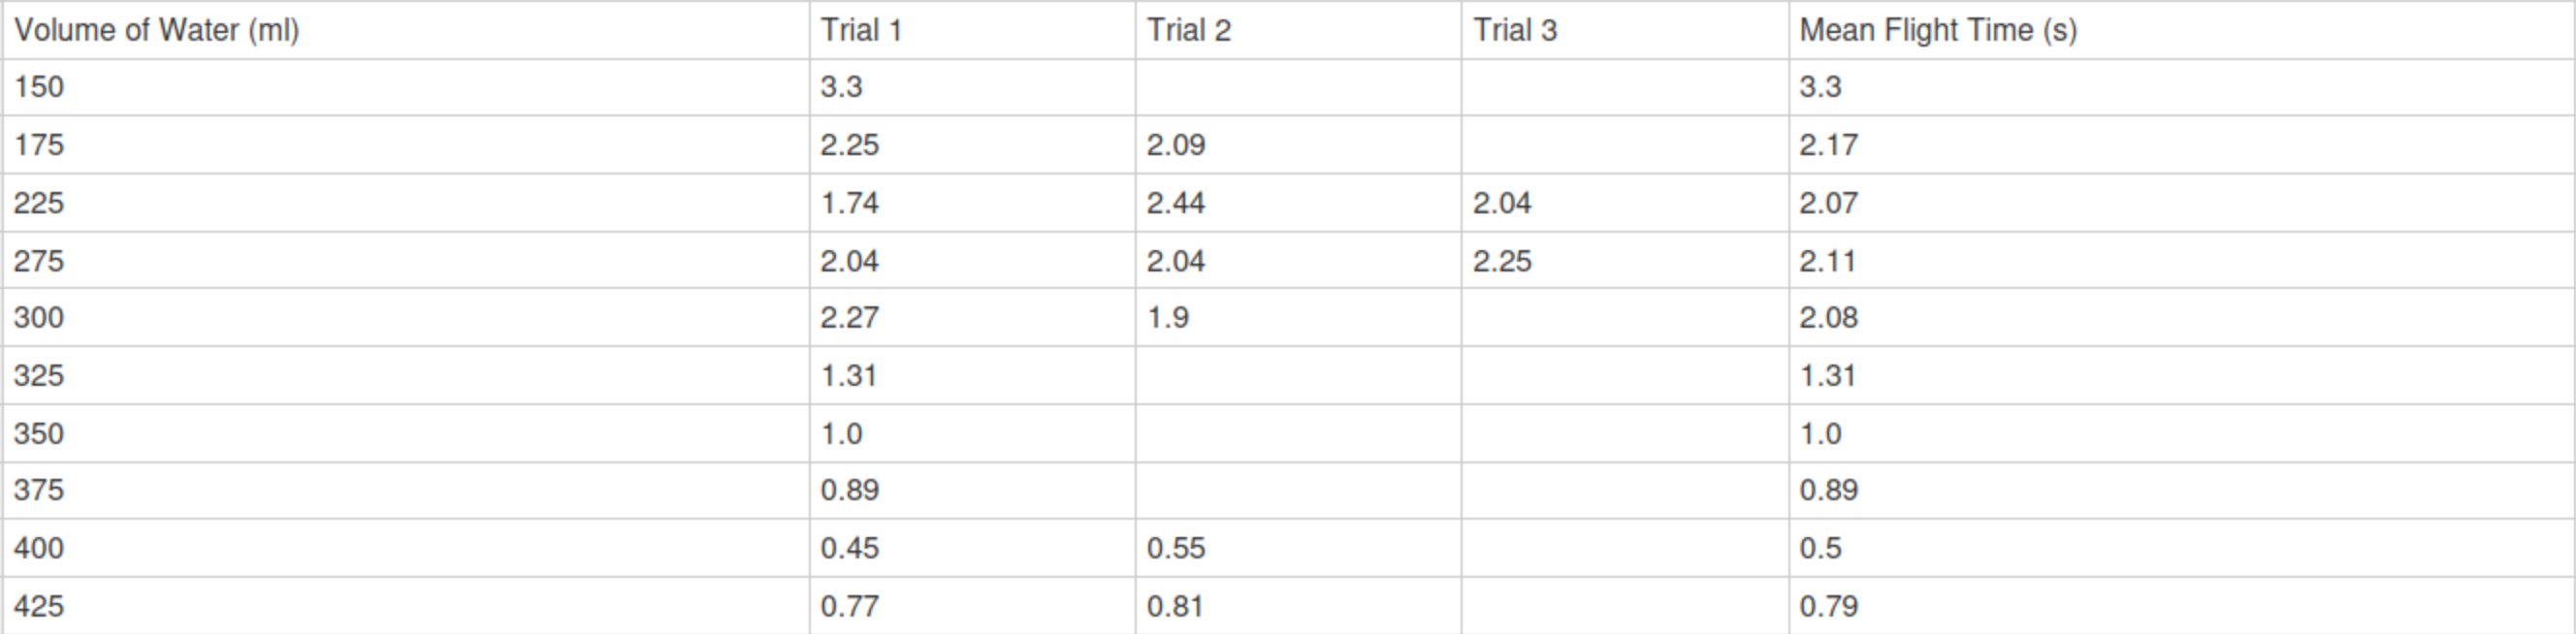
\includegraphics[width=\textwidth]{data/21st-30th.png}
\end{figure}
\FloatBarrier


\subsection{Appendix B}
\label {Appendix B}
The measurements we took of our rocket were:
\begin{itemize}
    \item Rocket Diameter = 70mm
    \item Rocket Nozzle Diameter = 26mm
    \item Bottle total volume = 1.052L
    \item Mass of the bottle = 39g
    \item Mass of the launch kit that is launched with the rocket = 19g
    \item Total rocket mass = 58g
\end{itemize}
\subsection{Appendix C}
\label {Appendix C}
Here is the code we pasted into the developer console on the website http://www.aircommandrockets.com/sim/simulator.htm
\begin{minted}{javascript}
// @ts-nocheck

function presetValues() {
  $("#rocketDiameter").val(70);
  $("#nozzleDiameter").val(26);
  $("#volume").val(1.052);
  $("#mass").val(58);
  $("#mass").val(58);
  $("#drag").val(0.5);
  $("#waterAmount").val(0.75);
  $("#pressure").val(1);

  try {
    $("#rocketDiameter").trigger("input").trigger("change");
  } catch (error) {}
  try {
    $("#nozzleDiameter").trigger("input").trigger("change");
  } catch (error) {}
  try {
    $("#volume").trigger("input").trigger("change");
  } catch (error) {}
  try {
    $("#mass").trigger("input").trigger("change");
  } catch (error) {}
  try {
    $("#mass").trigger("input").trigger("change");
  } catch (error) {}
  try {
    $("#drag").trigger("input").trigger("change");
  } catch (error) {}
  try {
    $("#waterAmount").trigger("input").trigger("change");
  } catch (error) {}
  try {
    $("#pressure").trigger("input").trigger("change");
  } catch (error) {}
}

function simulate() {
  let times = [];
  for (let i = 0.1; i <= 1; i += 0.01) {
    try {
      $("#waterAmount").val(i).trigger("input").trigger("change");
      $("#runSimBtn").trigger("click");
      let time = document.getElementById("crashdownTime").innerText;
      time = Number(time.slice(0, -2));
      times.push(time);
    } catch (error) {
      times.push(NaN);
    }
  }
  return times;
}

presetValues();
console.log(simulate().toString());
\end{minted}
We fed this into a python program that would generate a csv file and a graph based on the data.
\begin{minted}{python}
import matplotlib.pyplot as plt

volumes = [i/100 for i in range(10, 100)]
times = list(map(float, input("Enter the times: \n").split(",")))

with open("output.csv", "w") as file:
    file.write("Volume of water (l), Flight Time(s)\n")
with open("output.csv", "a") as file:
    for i, j in zip(volumes, times):
        file.write(f"{i}, {j}\n")

#print(times, volumes)

plt.plot(volumes, times, marker="x")
plt.ylabel("Flight Time (s)")
plt.xlabel("Volume of water (l)")
plt.grid(True)
plt.show()
\end{minted}
Here is the csv file generated:
\begin{minted}{python}
Volume of water (l), Flight Time(s)
0.1, 2.87
0.11, 2.97
0.12, 3.06
0.13, 3.13
0.14, nan
0.15, 3.26
0.16, 3.3
0.17, 3.34
0.18, 3.37
0.19, 3.4
0.2, 3.43
0.21, 3.45
0.22, 3.46
0.23, 3.47
0.24, 3.47
0.25, 3.47
0.26, 3.46
0.27, 3.45
0.28, 3.44
0.29, 3.42
0.3, 3.4
0.31, nan
0.32, 3.34
0.33, 3.3
0.34, 3.26
0.35, 3.22
0.36, 3.16
0.37, 3.13
0.38, 3.12
0.39, 3.11
0.4, 3.08
0.41, 3.05
0.42, 3.0
0.43, 2.95
0.44, 2.89
0.45, 2.81
0.46, 2.71
0.47, 2.62
0.48, 2.51
0.49, 2.36
0.5, 2.21
0.51, 2.08
0.52, 1.96
0.53, 1.85
0.54, 1.75
0.55, 1.65
0.56, 1.57
0.57, 1.49
0.58, 1.42
0.59, 1.35
0.6, 1.29
0.61, 1.24
0.62, 1.18
0.63, 1.13
0.64, 1.08
0.65, 1.04
0.66, 0.99
0.67, 0.95
0.68, 0.91
0.69, 0.88
0.7, 0.84
0.71, 0.81
0.72, 0.78
0.73, 0.74
0.74, 0.72
0.75, 0.69
0.76, 0.66
0.77, 0.63
0.78, 0.62
0.79, 0.59
0.8, 0.57
0.81, 0.55
0.82, 0.52
0.83, 0.51
0.84, 0.49
0.85, 0.47
0.86, 0.45
0.87, 0.43
0.88, 0.43
0.89, 0.41
0.9, 0.39
0.91, 0.38
0.92, 0.36
0.93, 0.35
0.94, 0.35
0.95, 0.33
0.96, 0.31
0.97, 0.31
0.98, 0.29
0.99, 0.3
\end{minted}
\end{document}
